\section{自製 GUI Framework}
\label{app:gui}

\subsection{設計動機與範圍}

這次作業沒有使用第三方 GUI framework，而是依照 drawing panel 的需要自行實作。我的目標不是做一套通用的桌面 toolkit，而是處理這個程式實際用到的多視窗、基本 control、Layout、focus、mouse capture、Event bubbling 與 OpenGL rendering。圖~\ref{fig:gui-classes} 顯示主要 class 之間的關係。

\begin{figure}[H]
    \centering
    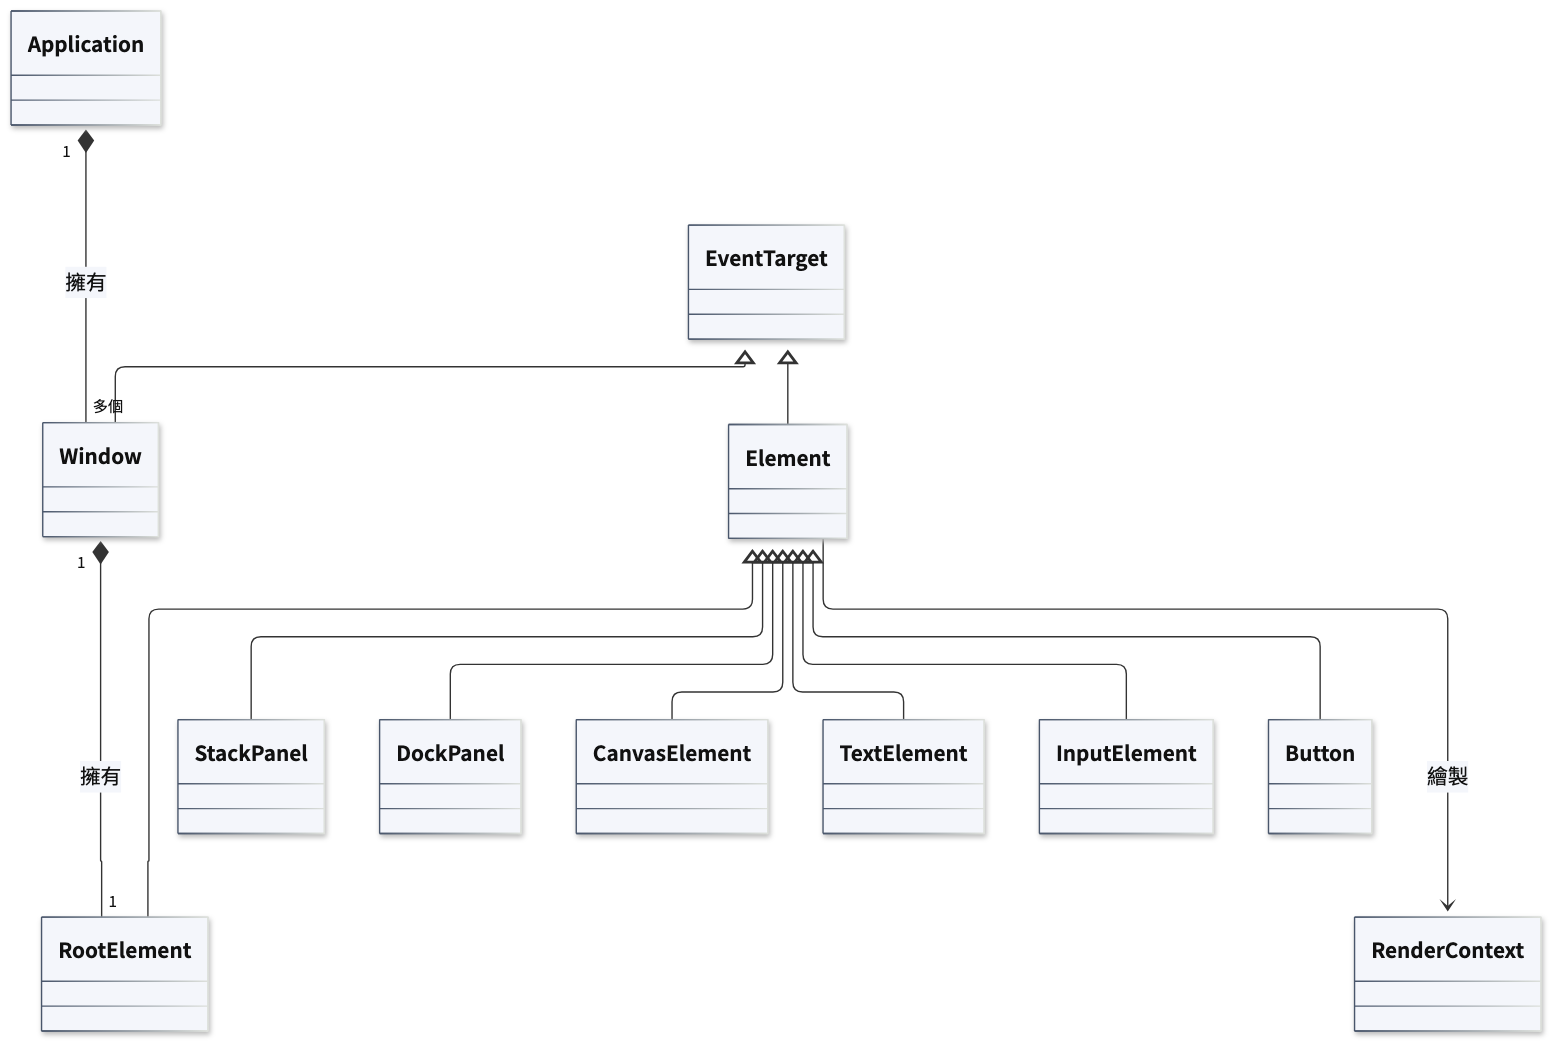
\includegraphics[width=.96\textwidth]{docs/figures/gui-classes.png}
    \caption{GUI 架構的主要類別關係}
    \label{fig:gui-classes}
\end{figure}

\subsection{Application 與 Window}

Application 建立並管理所有 Window。Window 內部記錄 GLUT window ID、大小、標題、RootElement、ColorBuffer 與互動狀態。每個 Window 都註冊相同的 static callbacks，再透過圖~\ref{fig:callback-routing} 的 ID 查找方式找回正確 instance。PaintWindow、InputDialogWindow、ConfirmWindow 與 GraphicsRenderWindow 都建立在這一層之上。

\subsection{Element Tree 與 Layout System}

每個 Element 記錄 parent、children、margin、padding、alignment 與 bounds。Layout 分成 measure 和 arrange 兩個階段：measure 先由下而上詢問每個元件需要多少空間，arrange 再由上而下分配實際位置。RootElement 只放一個主要內容；StackPanel 沿水平或垂直方向排列，並依 grow 權重分配剩餘空間；DockPanel 依加入順序從四邊扣除空間，最後一個 child 取得剩下區域。圖~\ref{fig:layout-tree} 是 PaintWindow 實際使用的 UI tree，圖~\ref{fig:layout-flow} 則整理從屬性變更到重新排版與繪製的流程。

\begin{figure}[H]
    \centering
    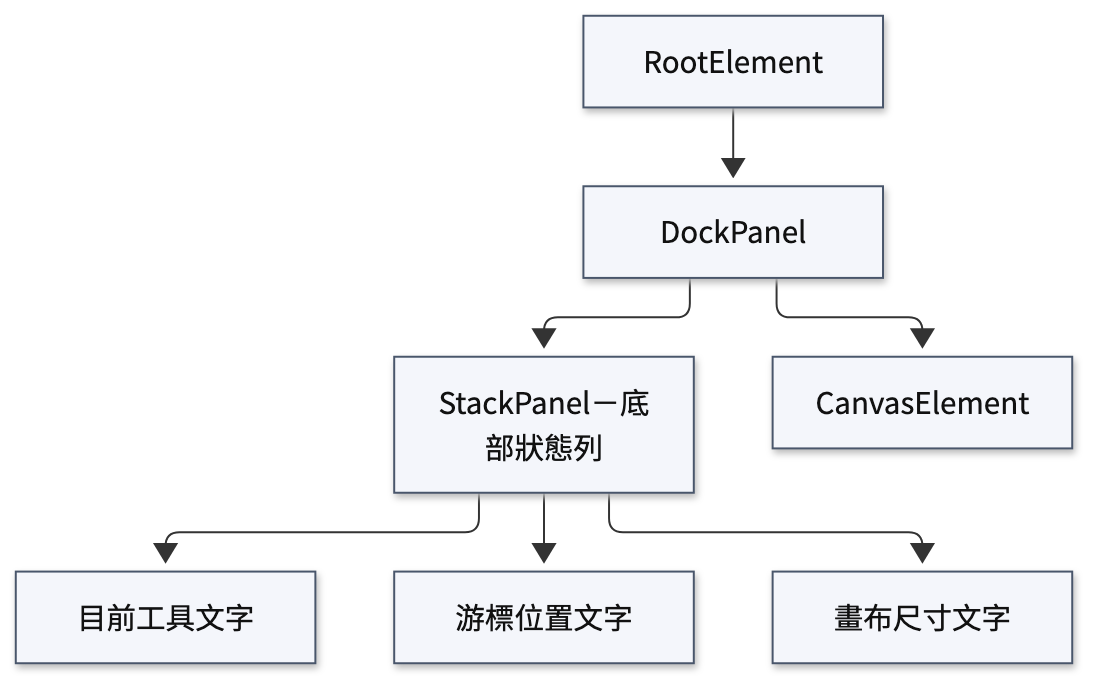
\includegraphics[width=.78\textwidth]{docs/figures/layout-tree.png}
    \caption{PaintWindow 的 Element 與 Layout 樹狀結構}
    \label{fig:layout-tree}
\end{figure}

\begin{figure}[H]
    \centering
    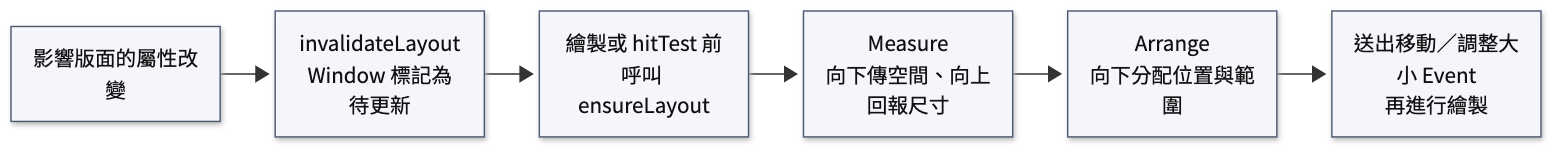
\includegraphics[width=.98\textwidth]{docs/figures/layout-flow.png}
    \caption{Element Tree 的測量、配置與重新繪製流程}
    \label{fig:layout-flow}
\end{figure}

當 preferred size、margin、padding 或 alignment 改變時，Element 會呼叫 \lstinline|invalidateLayout()|，再由所屬 Window 把 Layout 標成需要更新。下一次 render 或 hit test 前，Window 先呼叫 \lstinline|ensureLayout()|：measure 從 RootElement 往子節點傳入可用空間，子節點算完內容需求後再回報 desired size；arrange 則從視窗範圍開始，逐層分配實際 slot 與 bounds。這樣滑鼠命中測試使用的範圍會和畫面上實際繪製的位置一致。

\subsection{EventTarget、Bubbling 與 stopPropagation}

EventTarget 依 Event 型別記錄 listener。事件開始傳遞時，target 會保持為最初接收的元件，current target 則隨著 bubbling 一層一層改變。Element 會把事件傳給 parent，RootElement 再往上交給 Window。輸入框或快捷鍵處理完按鍵後，可以呼叫 \lstinline|stopPropagation()|，例如避免同一個 Enter 同時提交輸入框，又觸發上層 Window 的操作。傳遞流程見圖~\ref{fig:event-propagation}。

\subsection{Mouse Capture 與 Input State}

Window 會記錄目前取得 focus、hover 與 mouse capture 的 Element。MouseDown 後 Canvas 取得 capture，所以 Motion 與 MouseUp 仍會送回 Canvas；Hover 不受 capture 影響，繼續依游標實際位置更新。鍵盤狀態由視窗共用，滑鼠狀態則由各 Window 記錄。Modal Dialog 開啟或滑鼠進出視窗時，程式會清理相關狀態，避免按鍵或滑鼠按鈕一直停在按下狀態。

\subsection{Multi-window Lifecycle}

關閉 callback 不會立刻刪除 C++ object，而是先移除 GLUT ID，接著送出 WindowCloseEvent。PaintWindow 可以在這時檢查未儲存的修改並顯示 Confirm Dialog；使用者確定關閉後，Window 才會標記為可移除，最後由 Application 的 idle callback 釋放物件。Timer 每次執行前也會先確認視窗是否仍存在，避免 callback 執行到一半時物件已被銷毀。
